\documentclass[12pt]{article}

% Language setting
\usepackage[english]{babel}

% Set page size and margins
\usepackage[letterpaper,top=2cm,bottom=2cm,left=3cm,right=3cm,marginparwidth=1.75cm]{geometry}

% Useful packages
\usepackage{amsmath}
\usepackage{graphicx}
\usepackage[colorlinks=true, allcolors=blue]{hyperref}
\usepackage{sectsty} % For customizing section titles
\usepackage{xcolor}  % For color definitions
\usepackage{float}
\usepackage{graphicx}
\usepackage{url}


% Define Dark Blue color
\definecolor{DarkBlue}{rgb}{0, 0, 0.55}

% Set section title color to Dark Blue
\sectionfont{\color{DarkBlue}}

% Change the color of the document title to bold and Dark Blue
\title{\textbf{\textcolor{DarkBlue}{A Comparative Life-Cycle Assessment of Sustainable Aviation Fuel (SAF) Pathways}}}


\author{
    Aline Abayo \\ 
    Ahmed AlAli \\ 
    Marissa Marsh LoVullo \\ 
    Mohammed Rayes \\ 
    Oluwadamilare Hussein Orekoya
}
\date{}
\begin{document}
\maketitle

\begin{Appendix}
The aviation industry faces significant decarbonization challenges due to its heavy reliance on fossil-derived jet fuel. Sustainable aviation fuel (SAF) is a key strategy for reducing greenhouse gas (GHG) emissions in aviation and accelerating the progress towards zero-emission goals. This study evaluated the life-cycle GHG emission performance measured in grams of carbon dioxide equivalent per megajoule of SAF produced (gCO2e/MJ) and energy return on investment (EROI), the ratio of energy output to energy input (MJ/MJ) of two SAF production pathways: Hydroprocessed Esters and Fatty Acids (HEFA) from used cooking oil and soybeans and Alcohol-to-Jet (ATJ) from corn. The modeled ATJ scenarios did not achieve a 50\% reduction in GHG emissions compared to conventional aviation fuel, while the HEFA scenarios achieved 48\% to 83\% reduction in emissions. 
\end{abstract}

\subsubsection*{Keywords}Sustainable Aviation Fuel $|$ Life-Cycle Assessment $|$ Carbon Emissions $|$ Aviation Decarbonization

\section{Executive Summary}
This study conducts a comprehensive comparative life-cycle assessment (LCA) of three mature, sustainable aviation fuel (SAF) production pathways: Alcohol-to-Jet (ATJ), Fischer-Tropsch (FT), and Hydroprocessed Esters and Fatty Acids (HEFA). These alternative fuels are compared to conventional kerosene-based jet fuel to assess their environmental performance relative to the business as usual fuel source for the aviation industry in the United States (U.S.). The selected SAF pathways will be evaluated relative to conventional jet fuel concerning life-cycle GHG emissions, measured in units of grams of carbon dioxide equivalent per megajoule of SAF produced (gCO2e/MJ) and energy consumption in megajoules of energy per megajoule of SAF produced (MJ/MJ).

The International Civil Air Organization’s (2022) life-cycle assessment found that SAF pathways reduce GHG emissions compared to conventional jet fuel, but each SAF method has distinct trade-offs. ATJ does not result in the most significant reduction in emissions but utilizes existing crops and ethanol infrastructure. On the other hand, FT and HEFA, while generally offering more significant reductions in emissions, will perform differently based on feedstock sources and technological variations.

Critical to the analysis are the trade-offs inherent in different SAF production methods. While ATJ minimizes transportation network emissions due to corn abundance and existing infrastructure, corn fermentation requires significant quantities of water and energy. HEFA, reliant on lipid-based feedstocks, faces challenges related to feedstock availability. On the other hand, FT presents a flexible pathway using various biomass and waste feedstocks but requires more complex processing infrastructure. Such trade-offs and analyses are explored later in this study using the greenhouse gasses, regulated emissions, and energy use in transportation (GREET) model.

This study will examine mature SAF technologies and industry-relevant feedstocks in the U.S. The LCA scope of the ATJ process will focus on corn grain as feedstock and include cultivation, fermentation, upgrading, and transportation. The LCA for HEFA will specifically examine cooking oil as the feedstock, including fuel production and transportation. Lastly, an LCA of FT SAF with municipal solid waste as a feedstock and fuel production, transportation, and distribution stages are included in the scope. Emissions and energy from constructing related infrastructure are not included in the scope of this study; only emissions and energy to facilitate fuel production and transportation are examined. All the data contained in this study will be analyzed using GREET model assumptions.

\section{Introduction}
Aviation plays a crucial role in modern global transportation, but its environmental footprint is substantial due to its heavy reliance on petroleum-derived kerosene. Countries worldwide have stressed the importance of capping the rise in global temperature to 1.5 degrees Celsius by 2100 through the Paris Agreement (Lau et al. 2024). The aviation industry contributes approximately 2.5\% of global carbon dioxide (CO2) emissions, making it a key area to reduce emissions to meet international climate goals (Lau et al. 2024). The aviation sector is challenging to decarbonize for many reasons, including high fuel density requirements, weight and safety constraints, and the relatively high cost required to enter the aviation fuel market (Merchant et al. 2022). Approaches to reaching net-zero emissions in the aviation industry are synthetic fuels from biomass, fuels derived from green hydrogen and atmospheric carbon dioxide, and the direct use of green liquid hydrogen (Dray et al. 2022). One technologically mature solution to aviation’s emissions problem, sustainable aviation fuel (SAF), has high energy density and net heat of combustion that resembles the weight and volume characteristics of conventional aviation fuel (Wang & Rijal 2024).  
The International Air Transportation Association (2024) projects moving away from conventional aviation fuel and re-capturing CO2 emissions is critical to reaching net-zero emissions by 2050. SAF is derived from renewable resources, such as crops, agricultural waste, and used cooking oils. These feedstocks undergo chemical processes that make them chemically similar to traditional jet fuel, allowing them to be blended and used in existing aircraft without modifications. 
Two leading approaches to reducing carbon emissions associated with the aviation industry are mandating a carbon emission trading scheme and implementing the mandated use of SAF. Cui et al. (2023) systematically compared carbon emission trading schemes and the use of sustainable aviation fuel in Chain-foreign routes through projections of carbon dioxide and non-carbon dioxide emissions from 2023 to 2100. Their results show that SAF is more effective in controlling the pollutant emissions of aircraft than the European Union’s Carbon Emission Trading Scheme (EU ETS). However, the authors concluded that the most significant way to control emissions would be mandated SAF use and ETS policies to curb the effects of global climate change (Cui et al. 2023). These results highlight the importance of continuing research on the environmental impacts of SAF production as a favored solution in reaching net-zero emissions from aviation. 

In the United States, SAF development began with research and pilot projects by the U.S. Department of Energy and the Federal Aviation Administration in the early 2000s, focusing on alternative jet fuels. This culminated in ASTM International approving the first HEFA-based synthetic paraffinic kerosene in 2011, allowing up to a 50\% blend with conventional fuel. As of 2022, SAF accounted for less than 0.1\% of jet fuel consumed by the commercial aviation industry (U.S. Government Accountability Office 2023). Since then, SAF production has steadily increased, with a notable increase in domestic output from 5 million gallons in 2021 to 52 million gallons by mid-2024, and 11 SAF pathways have received ASTM International’s approval (Office of Energy Efficiency \& Renewable Energy 2024). 

Governments increasingly support the sector's decarbonization through fiscal support for SAF production and mandating SAF use. However, governments and international organizations are still developing specific decarbonization approaches to achieve net-zero aviation in 2050. The available literature on approaches to decarbonization heavily relies on SAF, which is not commercially available for the large-scale deployment required to meet net-zero goals. Additionally, the supply of necessary feedstocks for SAF production is insufficient for U.S. government goals for SAF production, given the current production technology (O’Malley et al. 2023). This research aims to support the development of comprehensive and informed policy recommendations to help organizations achieve their climate goals while ensuring continued economic growth and connectivity.


\section{Problem Statement}
Aviation’s dependency on fossil fuels makes it one of the most challenging sectors to decarbonize, with 2.5\% of global emissions attributed to this industry (Lau et al. 2024). While SAFs are a solution to reduce GHG emissions of aircraft, concerns about their life-cycle impact remain. This study addresses the need for a comparative evaluation of SAF pathways through a life-cycle assessment to understand their potential to mitigate aviation’s environmental impact.

\section{Questions to Answer}
\begin{itemize}
    \item How do ATJ, FT, and HEFA pathways compare with conventional jet fuel regarding life-cycle greenhouse gas emissions in grams of carbon dioxide equivalent per MJ of product and energy consumption?
    \item What are the trade-offs between different SAF production methods?
    \item What are the impacts of process type and location on SAF production in the United States on life-cycle greenhouse gas emissions?
    \item What are the critical environmental and economic challenges in scaling SAF production?
    \item Is there enough feedstock in the U.S. to produce SAF to supply the aviation industry?
\end{itemize}

\section{Background}



Recent literature has evaluated potential pathways to achieve decarbonization in the aviation industry. SAF is commonly viewed as one of the strategies to reach net-zero emissions as demand for aviation is expected to grow. 

Sacchi et al. (2023) quantified the efforts needed to mitigate the contribution of the European aviation fleet to global warming through a mixture of approaches. The study found that if aviation growth is sustained, fully mitigating the climate impacts caused by the European aviation sector will simultaneously require extensive Carbon Dioxide Removal (CDR), SAF, and other physical and market-based interventions that require significant energy, natural, and financial resources. In addition, the study suggests reducing air traffic demand is a good short- to mid-term solution while dually investing in the development of SAF and CDR (Sacchi et al. 2023).


In addition, Borgero et al. (2023) modeled the pathway to net-zero emissions. The researchers concluded that decarbonizing aviation will require large quantities of SAFs. The results suggested that an exponential growth of ethanol and biodiesel industries would be required to produce the 19.8 Exajoules of SAF necessary to achieve net-zero carbon emissions under business-as-usual (BAU) conditions in demand and energy intensity. Furthermore, the study underscored the uncertainty in the effects of aviation’s non-CO2 radiative forcing. Achieving a net-zero emissions sector would also rely on CDR ranging from 0.2 to 3.4 gigatonnes of CO2. They noted that if market-based mechanisms are less expensive than SAFs, airlines may seek to offset rather than reduce their combustion emissions; this argument emphasized the need to consider the cost-effectiveness of SAF production. 

Due to their identical chemical properties to kerosene, SAF is a “drop-in” fuel and a near-term solution for reducing aviation emissions. Pathways for SAF need to be approved by ASTM International to be blended with conventional fossil kerosene and interchangeable with existing infrastructures and jet engines (International Aviation Trade Association 2022). Therefore, existing aviation infrastructure can remain in place while new production and blending facilities are developed to increase fuel use. 

There are several production and conversion pathways to produce SAF and a wide variety of possible biofuel feedstocks. To date, the ASTM has certified eleven conversion pathways. Alcohol-to-jet (ATJ) and hydroprocessed esters and fatty acids (HEFA) pathways are among the most mature, well-researched and commercially viable production processes for sustainable aviation fuels (International Aviation Trade Association, 2024). Other pathways include the following methods: Fisher Troscp (FT), FT-based pathways containing aromatics feedstocks (FT-SKA), hydroprocessed fermented sugars (SIP), isobutanol and ethanol alcohol-to-jet (ATJ), catalytic hydrothermolysis jet (CHJ), hydrocarbons HEFA (HC-HEFA), co-hydroprocessing of FT hydrocarbons in a conventional petroleum refinery, and co-hydroprocessing of esters and fatty acids in a convention petroleum refinery (International Civil Air Organization 2022). Calderon et al. (2024) note that not one pathway will be able to meet all the SAF demand; instead, a composition of multiple pathways and feedstocks is necessary to meet the aviation industry’s projected demand. However, due to data availability constraints, we were unable to include analysis for all the pathways. 


The following sections expand on conventional aviation fuels as well as the two most technologically mature SAF production pathways: hydroprocessed esters and fatty acids (HEFA) from used cooking oil and soybeans and alcohol-to-jet (ATJ) from corn. The background information from existing literature and the life-cycle of each fuel type is discussed.


\subsection{Conventional Aviation Fuel }

\begin{figure}[H]
\centering
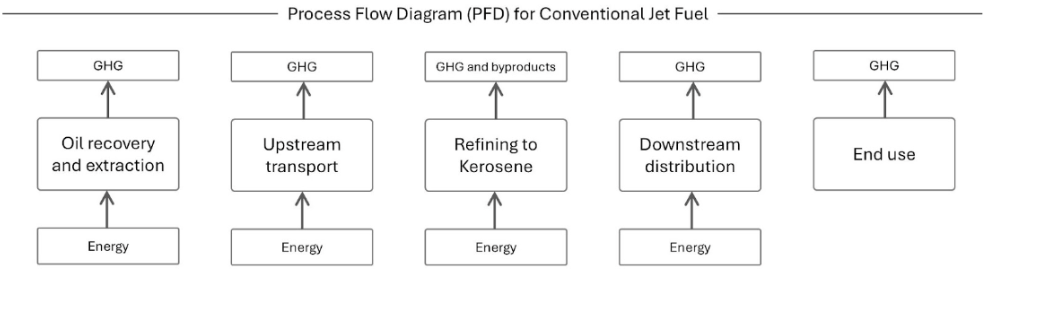
\includegraphics[width=0.8\textwidth]{Fig 1.png} % Replace 'fig10.png' with the path to your image file
\caption{A schematic overview of the conventional jet fuel supply chain and process flow diagram (PFD) used in this study}
\label{fig:figure 1}
\end{figure}

In the United States, the well-to-wake (WTW) life-cycle of jet fuel (kerosene) used in the aviation industry is produced through several key stages illustrated in Figure 1: extraction, refining, transportation, storage, distribution, and combustion. Each stage contributes to greenhouse gas (GHG) emissions. These emissions are presented in units of CO2e, which accounts for CO2 and other gas emissions expressed at the 100-year global warming potential from energy consumption throughout the life-cycle. This report will provide a detailed breakdown of emissions for each stage of the kerosene WTW life-cycle, as per a study by Jing et al. (2022). International Civil Air Organization’s (2022) (ICAO) life-cycle assessment methodology was also used for comparison. 
\begin{table}[h!]
\centering
\begin{tabular}{|c|c|}
\hline
\textbf{LCA Stage} & \textbf{gCO2e /MJ} \\
\hline
Drilling and Extraction & 9.6 \\
Refining and Distillation & 4.5 \\
Transportation of Kerosene & 0.8 \\
Storage of Kerosene & 0.1 \\
Distribution of Kerosene & 0.8 \\
Combustion & 73.8 \\
\hline
\textbf{Total} & \textbf{89.6} \\
\hline
\end{tabular}
\caption{The total well-to-wake emissions for kerosene in the U.S. are 89.6 gCO2e/MJ, adapted from Jing et al. 2022.}
\label{tab:kerosene_emissions}
\end{table}

Extraction is one of the most energy-intensive stages of the kerosene life-cycle in the U.S., contributing 9.6 gCO2e/MJ of fuel produced to the overall emissions. This reflects the emissions from energy consumption and associated activities from onshore and offshore drilling. The U.S. emissions are relatively high due to the heavy crude oils extracted and the more energy-intensive recovery processes. For example, in Saudi Arabia, emissions in the extraction stage are much lower due to lighter crude oils and more efficient extraction technologies (Jing et al. 2022).

Refining in the U.S. results roughly in 4.5 gCO2e/MJ (Jing et al. 2022). While ICAO’s Carbon Offsetting and Reduction Scheme for International Aviation (CORSIA) model estimates refining to produce 1.7 gCO2e/MJ, this number is underestimated and biased since it was obtained from U.S. oil refineries (ICAO 2022). The refining stage involves fractional distillation, a process in which crude oil is heated and hydrocarbon products are separated, resulting in refined kerosene. U.S. refineries often use energy- and time-intensive deep conversion processes due to the need to process heavier crude oils. In contrast, countries like Saudi Arabia process lighter crude oil, which results in lower emissions during the refining stage. China and the European Union exhibit refining emissions similar to those of the U.S., mainly due to the complexity of the crude oil they process (Jing et al. 2022).

Once refined, kerosene is transported to distribution centers via pipelines, trucks, and rail. The transportation stage in the U.S. adds 0.8 gCO2e/MJ to the life cycle emissions. This reflects the energy used to move kerosene across large distances in the U.S., a vast country with dispersed consumption points. In comparison, Saudi Arabia, with its more centralized refining and distribution infrastructure that mainly relies on pipelines, experiences lower transportation emissions (Jing et al. 2022).

Kerosene is stored at various terminals and airports before use. The storage stage has relatively low emissions, contributing about 0.1 gCO2e/MJ (ICAO 2022). Emissions from storage are associated with maintaining the product at bulk plants using storage tanks (Jing et al. 2022).

Since storage tanks are closed roof systems, emissions rarely escape. Fugitive emissions typically appear in the truck loading stage, where trucks are being refueled for distribution.
The distribution of kerosene from storage terminals to airports results in an additional 0.8 gCO2e/MJ of emissions. Similar to transportation, this stage is influenced by the U.S.'s geography, where kerosene must be transported over long distances to reach major airports. Regions with smaller geographic areas, more centralized refining, and heavy reliance on pipeline distribution show lower distribution emissions (Jing et al. 2022).

The final and most significant contributing stage of the kerosene life-cycle is its combustion in jet engines during air cruising. The combustion of kerosene emits 73.8 gCO2e/MJ, which is by far the largest contributor to the total life-cycle emissions. This accounts for the majority of greenhouse gases released. This figure is consistent globally, as jet fuel combustion processes are similar across countries. The U.S. total well-to-wake emissions for kerosene stand at 90.8 gCO2e/MJ, slightly above the global average of 88.7 gCO2e/MJ (Jing et al. 2022).

The extraction and combustion stages primarily drive the life-cycle kerosene emissions in the U.S. The total emissions of U.S. kerosene at 89.6 gCO2e/MJ is slightly higher than the global average due to the heavier crude oils processed and the energy-intensive refining practices. CORSIA’s model presents the U.S. results as 84.3 gCO2e/MJ, which, as mentioned earlier, the data source is biased (ICAO 2022). Comparing these figures to other regions, Saudi Arabia demonstrates the lowest emissions at 81.1 gCO2e/MJ, mainly due to its more efficient extraction and refining processes. The EU and China present values similar to those of the U.S., at 89.1 gCO2e/MJ and 89.7 gCO2e/MJ, respectively. Reducing U.S. kerosene life-cycle emissions should focus on improving refinery efficiency and exploring alternatives to fossil-based jet fuels. The high emissions from aircraft fuel combustion highlight the need for fuel alternatives like SAF, improved engine efficiency, and operational measures such as optimized flight paths to reduce aviation's environmental impact (Jing et al. 2022).

\subsection{SAF Production Pathways}

\begin{figure}[H]
\centering
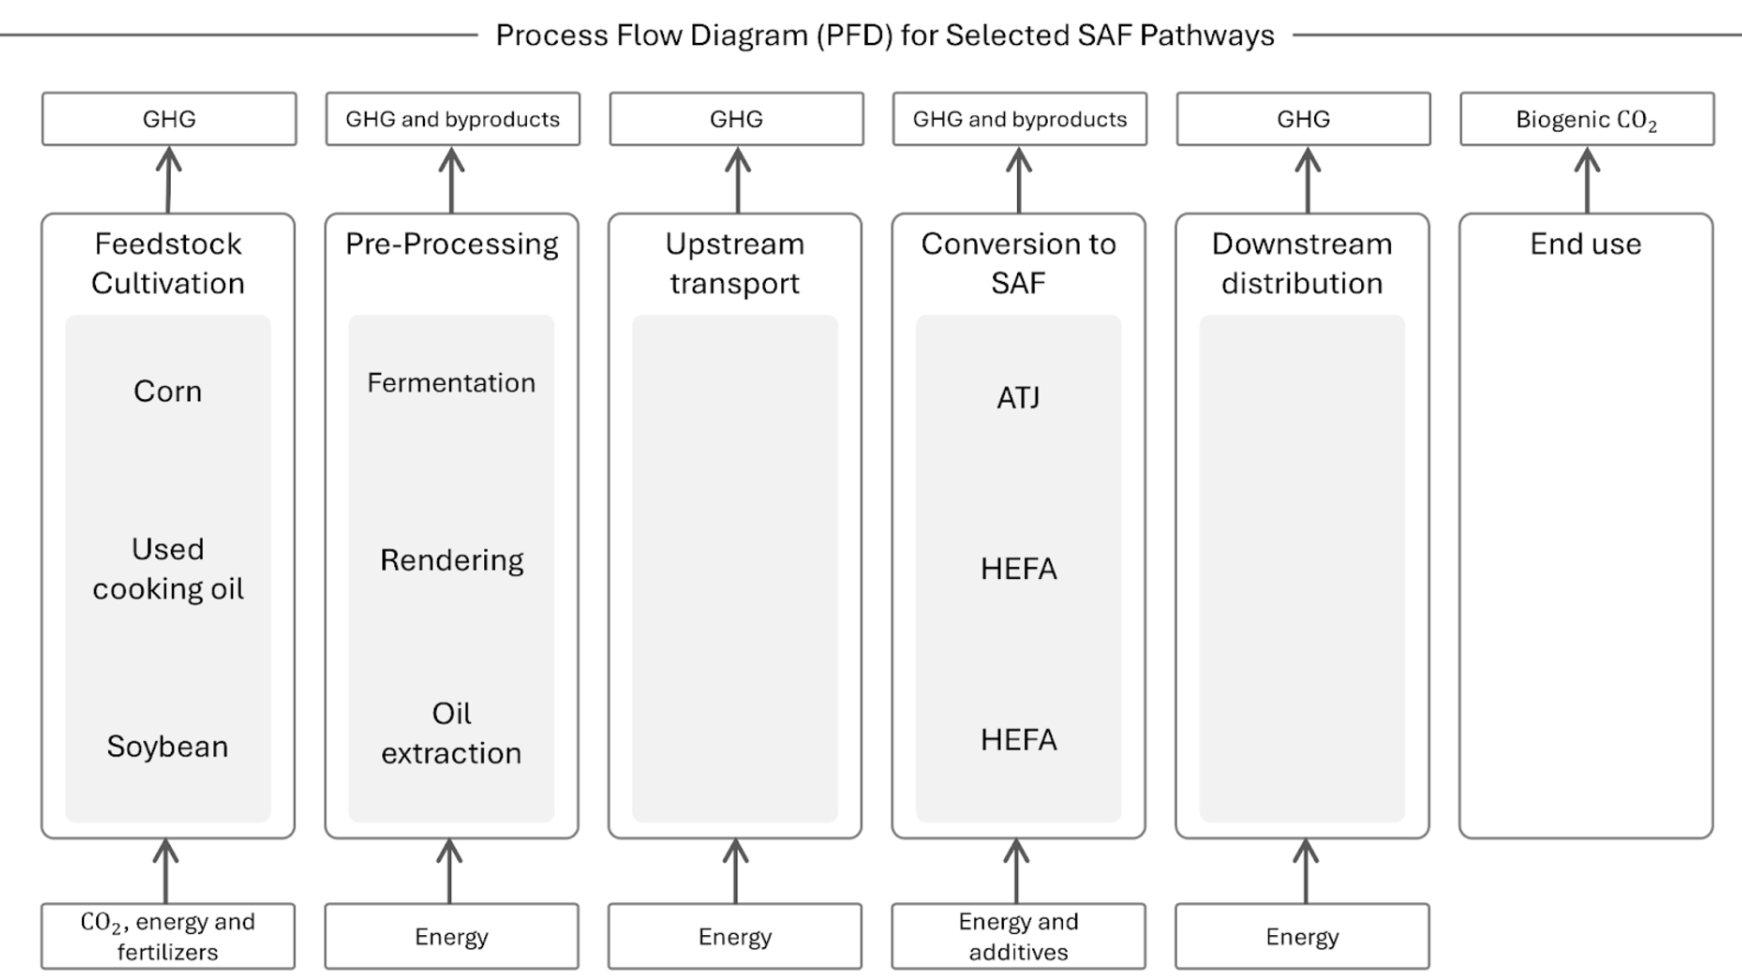
\includegraphics[width=0.8\textwidth]{Fig 2.png} % Replace 'fig10.png' with the path to your image file
\caption{A schematic overview of selected SAF pathways supply chain and the process flow diagram (PFD) used in this study}
\label{fig:figure 2}
\end{figure}

There are various ways to produce SAF from different production pathways and feedstocks. Stakeholders in the SAF industry state that the availability of SAF feedstocks is one of the top constraints of the industry’s growth (Calderon et al. 2024). Depending on geographic resource availability and demand, a combination of pathways and sustainable feedstocks may meet regional demand for SAF while minimizing the industry’s climate footprint.

\subsubsection{HEFA}

Hydroprocessed Esters and Fatty Acid (HEFA) fuel is the market's most widely available and commercially viable SAF (Calderon et al. 2024). It has the highest energy conversion efficiency of the SAF pathways at 76\% (Lau et al. 2024). The life-cycle GHG emissions of HEFA SAF are approximately 27 to 55 gCO2e/MJ of SAF produced depending on the feedstock (de Jong et al. 2017). A low-carbon electricity grid and renewable hydrogen can further lower the fuel's carbon footprint. Mannion et al. (2024) compared embodied GHG emissions from current literature on HEFA feedstocks, which are included in the figure below. Unknown UCO refers to the uncertainty in the exact composition of waste cooking oil as a SAF feedstock in the figure below. 

\begin{figure}[H]
\centering
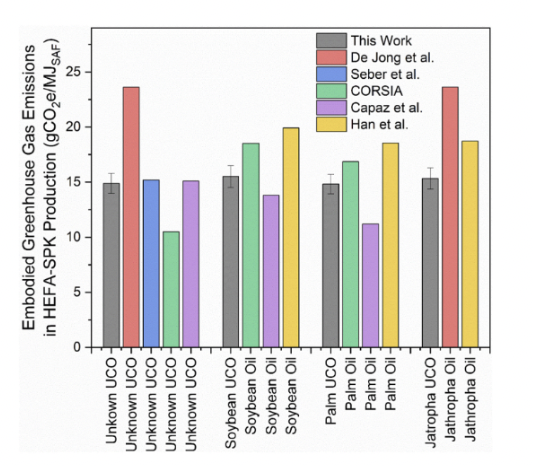
\includegraphics[width=0.8\textwidth]{Fig 3.png} % Replace 'fig10.png' with the path to your image file
\caption{Comparison of embodied emissions in HEFA feedstocks from existing literature reproduced from Mannion et al. 2024}
\label{figure 3}
\end{figure}

HEFA fuels are produced from various feedstocks. The following feedstocks are eligible for the 40B Provision of the Inflation Reduction Act’s sustainable aviation fuel credit: U.S. soybeans, U.S. and Canadian canola oil, used cooking oil, tallow, and distillers corn oil (Wang et. al 2024). The production of SAF by the HEFA pathway is limited by the availability of feedstocks, which considerably influences the fuel price due to the feedstocks' rising cost as demand from the biofuel industry grows (Lau et al. 2024). Algae oil is an emerging feedstock for HEFA SAF, but the Department of Energy projects that the feedstock may reach full-scale deployment around 2040 to 2050 (Calderon et al. 2024). 

\begin{figure}[H]
\centering
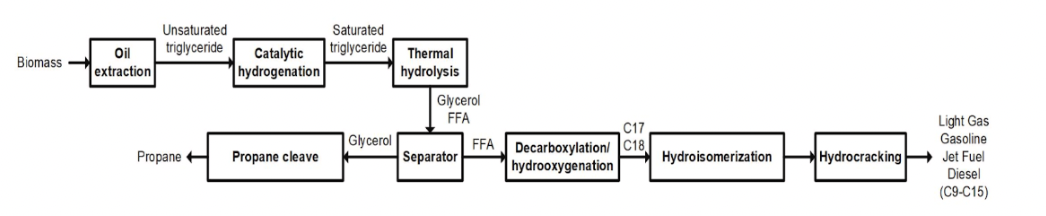
\includegraphics[width=0.8\textwidth]{Fig 4.png} % Replace 'fig10.png' with the path to your image file
\caption{HEFA production process reproduced from Lau et al. 2024}
\label{figure 4}
\end{figure}
The ASTM International approved Hydroprocessed Esters and Fatty Acids-Synthetic Paraffin Kerosene as an aviation fuel with a maximum percent blend rate of 50\% with conventional jet fuel. The HEFA process extracts oil from the biomass feedstock and transforms it through several chemical processes to become SAF. Feedstocks like wastes and animal fats are pretreated to remove impurities before refinement. Next, unsaturated fatty triglycerides are heated and hydrogenated with nickel, palladium, or platinum catalysts (Lau et al. 2024). The saturated triglycerides then go through thermal hydrolysis reactions to be broken down to glycerol that can produce propane and free fatty acids for further refinement to fuel (Lau et al. 2024). Next, the free fatty acids undergo decarboxylation or hydroxygenation at 300 to 600 degrees Celsius (Lau et al. 2024). A significant amount of hydrogen atoms are added as a catalyst to remove oxygen from the fats and oils, producing a pure hydrocarbon through the hydrodeoxygenation process (Wang et al. 2024). To lower the fuel’s freezing point, the pure hydrocarbons undergo hydroisomerization, coinciding with or after the hydrocracking process to produce SAF to meet ASTM properties suitable for flying at high altitudes (Lau et al. 2024). 

\begin{figure}[H]
\centering
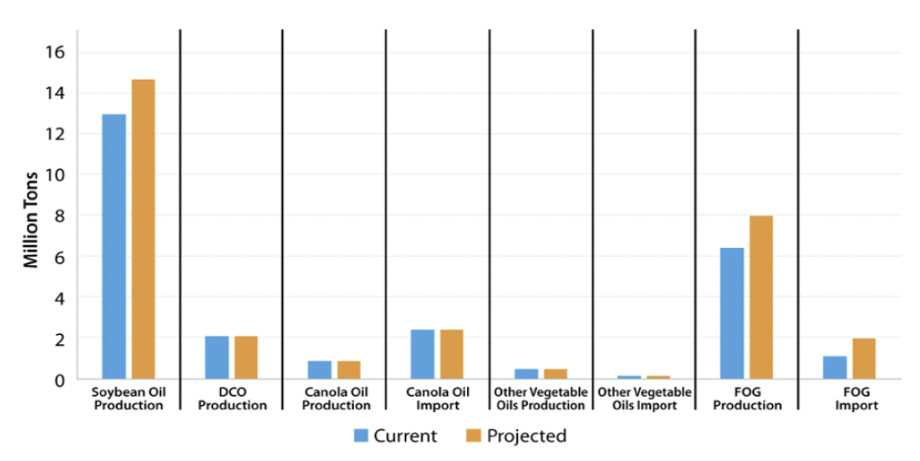
\includegraphics[width=0.8\textwidth]{Fig 5.png} % Replace 'fig10.png' with the path to your image file
\caption{Current and projected HEFA feedstock supply (2030-2032) reproduced from Calderon et al. 2024}
\label{figure 5}
\end{figure}


Used cooking oil (UCO), which also referred to as fats, oils, and greases (FOG) when combined with animal tallow and collected grease from wastewater facilities, is the second most abundant feedstock in the U.S. and has been evaluated for this comparative LCA for the HEFA pathway. The feedstock consists of UCO from commercial and industrial cooking operations unsuitable for human consumption (Calderon et al. 2024). Because UCO wastes are produced from various sources, a specific sample of the feedstock can be highly variable in terms of fatty acid content, thus resulting in differing energy conversion efficiencies (Mannion et al. 2024). The current production of UCO is estimated to be 1.4 million tons, geographically distributed throughout the country, with the highest production mirroring high population densities (Calderon et al. 2024).  Soybean oil is the most abundant feedstock in the US, and due to increased domestic market demand for soybean oil, soybean exports have declined 70\% over the last ten years (Calderon et al. 2024). Some biofuel producers prefer using inedible feedstocks like used cooking oil and tallow over crops for food production, like Neste, which only uses waste products for feedstocks (Calderon et al. 2024). Technological advancements and ground transportation electrification may result in more HEFA feedstock availability for SAF as facilities switch production from renewable diesel to SAF (Calderon et al. 2024). 


\subsubsection{ATJ}

 The Alcohol-to-Jet (ATJ) process allows for the sustainable production of kerosene from ethanol. Growing feedstocks for fuel production involves carbon sequestration, which offsets the CO2 produced by combustion in later stages. ATJ typically converts alcohols, such as ethanol or butanol, into synthetic paraffinic kerosene, chemically identical to conventional jet fuel. The ATJ process is especially viable in regions like the United States, where corn grain is a primary feedstock for ethanol production. Corn accounts for 53.7\% of global ethanol production, making it a cornerstone in biofuel initiatives (Lau et al. 2024). The U.S. is the world’s largest producer of corn, offering a consistent and reliable domestic supply that is rarely affected by external uncertainties. Although more efficient processes such as Hydroprocessed Esters and Fatty Acids (HEFA) and Fischer-Tropsch (FT) are also used in the SAF landscape, ATJ remains a popular choice due to its compatibility with the vast ethanol production infrastructure in the U.S. 
 
\begin{figure}[H]
\centering
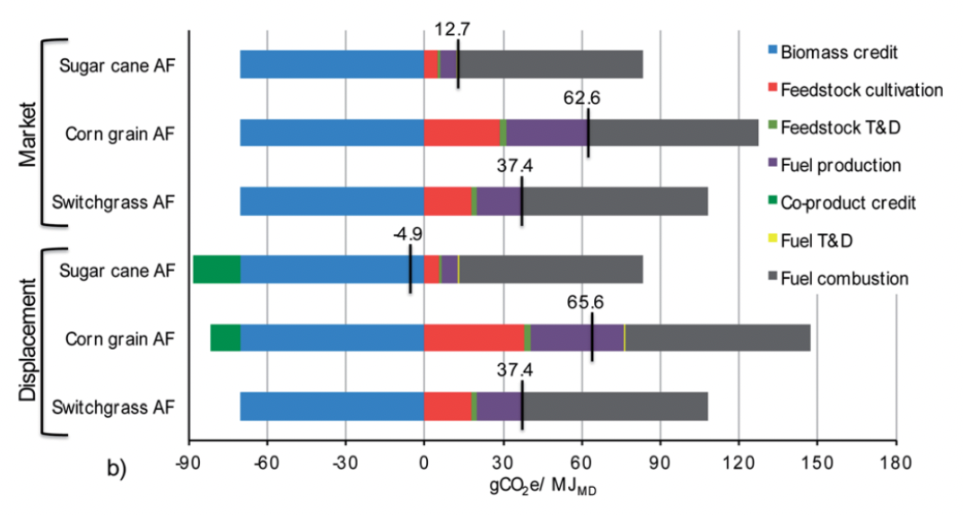
\includegraphics[width=0.8\textwidth]{Fig 6.png} % Replace 'fig10.png' with the path to your image file
\caption{Life-cycle GHG footprint breakdown reproduced from Staples et al. 2014}
\label{figure 6}
\end{figure}


 The life-cycle of ATJ fuel consists of the following stages: feedstock growth, feedstock cultivation, fuel production, and combustion. Growing the feedstock for ATJ is a carbon sequestration process that provides a “biomass credit” or negative CO2 emissions. For corn, feedstock growth is valued at around -75 gCO2/MJ. Next are the most energy-intensive processes of cultivation and fuel production. Cultivation is the stage at which land is prepared for growing crops, including soil preparation, weed control, water use, and soil aeration. This stage is one of the most energy-intensive steps in “Corn-To-Jet” alongside fuel production. Fuel production includes biorefining corn into ethanol and upgrading ethanol, which is turned into jet fuel. There are four major steps in fuel production: dehydration, oligomerization, hydrogenation, and distillation. While hydrogenation is not an energy-intensive process, the hydrogen used in this step is largely produced via steam methane reforming (SMR), which is energy-intensive (International Energy Agency, 2019).  The cultivation process produces 37.4 gCO2/MJ, while the fuel production process produces around 40 g CO2/MJ. These values are summarized in Figure 6 above from Staples et al. (2014). Adding up the emissions from the life-cycle stages of corn-grain ethanol yields a value of 65.6 gCO2/MJ, the agreed default core LCA value for corn-grain ethanol (ICAO 2022).

 While corn grain dominates U.S. ethanol production, there is future potential for using cellulosic feedstocks such as corn stover, switchgrass, and agricultural residues to produce cellulosic ethanol. These feedstocks are derived from the non-edible parts of plants, such as the stalks, leaves, and husks, making them a more environmentally friendly option than food crops like corn grain. The appeal of cellulosic ethanol lies in its potential to reduce land-use competition between food and fuel, lower GHG emissions, and increase the overall sustainability of biofuel production. However, the economical scale production of cellulosic ethanol is not yet feasible and depends on many constantly changing factors, such as crop and energy prices. It also requires technological advancements and policy changes before it can be considered reliable (Aui et al. 2024). Figure 7 below shows the potential reduction of CO2 emissions when comparing conventional jet fuel to SAF sourced from corn grain and corn stover feedstocks. Moving from corn grain to corn stover feedstocks offers 49.5 gCO2e/MJ reduction in emissions (Han et al. 2017). 

\begin{figure}[H]
\centering
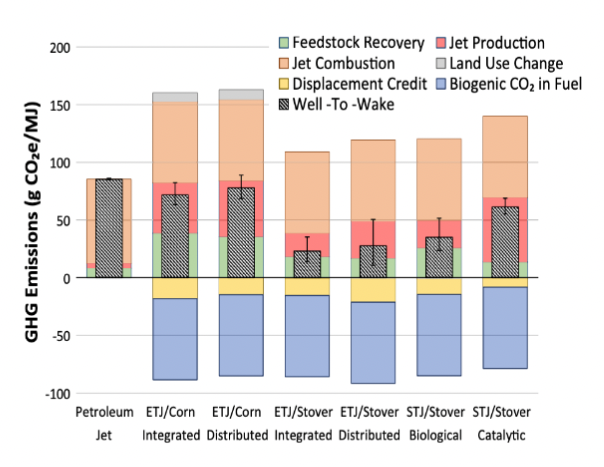
\includegraphics[width=0.8\textwidth]{Fig 7.png} % Replace 'fig10.png' with the path to your image file
\caption{WTWa GHG emissions of ETJ and STJ compared to petroleum jet reproduced from Han et al. 2017}
\label{fig:figure 7}
\end{figure}
 
\subsubsection{FT}

Fischer-Tropsch (FT) synthesis is among the most established and widely researched technologies for producing SAF. Among the feedstocks for FT synthesis, municipal solid waste (MSW) presents a promising resource, particularly when landfill gas (LFG) is captured and converted into fuel. The use of MSW reduces the reliance on fossil fuels and is also a mitigation solution for methane emissions from landfills, which has been a challenging sector to decarbonize. As shown in Figure 8, landfills were the third-largest source of human-related methane emissions in the United States in 2022 (Environmental Protection Agency 2024).

Though there are various options for converting LFG into energy—including electricity generation, direct use of medium-Btu gas, and renewable natural gas—these approaches are often limited by low energy conversion efficiencies, high GHG emissions, and high maintenance costs, often requiring substantial subsidies. Converting LFG to SAF offers an alternative opportunity for achieving higher energy conversion efficiency while mitigating methane emissions more effectively, reducing GHG impacts, and creating a valuable low-carbon fuel. This pathway can thus play a significant role in both sustainable aviation fuel production and broader climate mitigation efforts (Pressley et al. 2014). 

\begin{figure}[H]
\centering
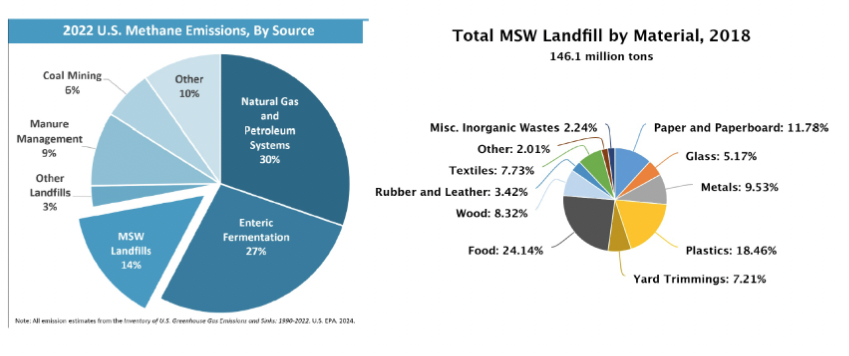
\includegraphics[width=0.8\textwidth]{Fig 8.png} % Ensure this filename matches exactly
\caption{2022 US Methane Emissions by sources (left) reproduced from Environmental Protection Agency n.d. (left), and MSW landfill material composition 2018 reproduced from Environmental Protection Agency n.d. (right)}
\label{figure8}
\end{figure}

MSW differs from other biomass-to-fuel feedstock sources. This is because MSW has a pre-existing life-cycle that is altered when it is used as fuel feedstock, whereas in the case of crop-based biomass, additional feedstock is cultivated for fuel production. Therefore, the scope of this analysis excludes the processes irrespective of the waste management, such as collection and existing sorting for recycling and composting. Therefore, the system boundary does include the effects of eliminating waste management processes such as landfill and accounts for the impacts of MSW conversion to MD fuels and their end-use (Suresh et al. 2018).

\begin{figure}[H]
\centering
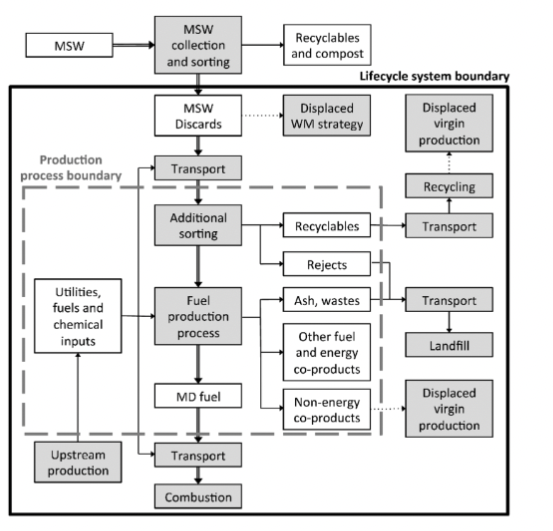
\includegraphics[width=0.8\textwidth]{Fig 9.png} % Ensure this filename matches exactly
\caption{Life-cycle GHG emissions system boundary reproduced from Suresh et al. 2018}
\label{figure8}
\end{figure}

Using the methodology by Suresh et al. (2018), the LCA begins when MSW discards exit the sorting facility, incorporating only these discards after recycling and composting have been separated.  In addition, the LCA includes the impact of displacing the existing waste management strategy in the U.S. Within this boundary, the analysis captures the transport of the feedstock to the production plant, preprocessing to remove non combustibles, and the conversion process that generates fuel and coproducts, such as excess electricity and aggregates. Waste streams from production, including ash and spent catalysts, are disposed of in landfills. The final stages of the system boundary encompass the transportation, distribution, and combustion of the produced fuel (Suresh et al., 2018)

\begin{figure}[H]
\centering
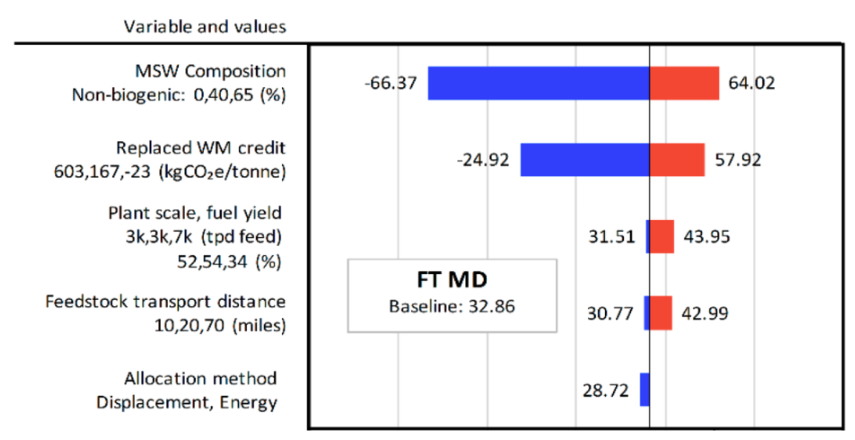
\includegraphics[width=0.8\textwidth]{Fig 11.png} % Replace 'fig11.png' with the path to your image file
\caption{Life-cycle GHG emissions sensitivity analysis showing the resultant median value reproduced from Suresh et al. 2018}
\label{fig:figure11}
\end{figure}

In addition, another MSW-to-SAF feasibility study done for King County, Seattle, showed that MSW to SAF via FT is a promising technology with the potential to reduce greenhouse gas emissions, divert waste from landfills, and build regional economies. However, the authors reiterate that financing for waste-to-fuel conversion projects is more challenging than for established, proven industrial projects. SAF projects face higher technology and permitting risks, which must be addressed and mitigated to attract investors. In addition, at the time of the study, some programs did not consider MSW as a renewable feedstock, which resulted in significantly different lifetime GHG emissions calculated using the respective formulas for calculating the carbon intensity. At the time, the GREET model did not have a published procedure for accounting for the MSW to SAF conversion process emissions. Now, these figures are available in GREET, making it a critical time to revisit the MSW to SAF via FT conversation. (EXP 2023)

\subsubsection{ U.S. Government Initiatives}

The U.S. Department of Energy, Department of Transportation, and Department of Agriculture launched the SAF Grand Challenge to accelerate the growth of SAF to decarbonize the aviation industry. The U.S. government seeks to reach 3 billion gallons of domestic SAF production per year by 2030 and 35 billion gallons of production per year by 2050 to meet aviation’s domestic fuel demand, given that the fuel results in a minimum reduction of greenhouse gas emissions of 50\% compared to conventional fuel (Office of Energy Efficiency \& Renewable Energy 2024). The agencies have coordinated a voluntary reporting system to track progress toward the stated goals. Additionally, the above agencies and the Federal Aviation Administration have funded \$443 million in various research and development projects, including feedstock supply chain development, ASTM International investment, and SAF commercial deployment (Office of Energy Efficiency \& Renewable Energy 2024). 

This year’s SAF production is estimated to be 52 million gallons as of June 2024, predominantly from fat, oil, and grease feedstocks through the HEFA pathway (Office of Energy Efficiency \& Renewable Energy 2024). Domestic SAF production has risen from 5 million and 26 million gallons in 2021 and 2023, respectively (Office of Energy Efficiency \& Renewable Energy 2024). The Department of Energy estimates that SAF production last year reduced 154,000 to 216,000 metric tons of CO2e, based on an assumed 50\% to 70\% reduction from the HEFA production pathway (Office of Energy Efficiency \& Renewable Energy 2024). Based on the planned SAF projects, the coalition is optimistic that the domestic market will meet the 2030 production goal. 

\subsubsection{SAF Feedstock Availability}

The International Council on Clean Transportation estimated that the U.S. will have 12.2 billion gallons of SAF available from sustainably sourced domestic feedstocks by 2050 (O’Malley et al. 2023). Soybean oil and corn grain ethanol did not meet the 50\% life-cycle GHG emission reductions required by the 40B tax credit for the SAF Grand Challenge goals (O’Malley et al. 2023). The breakdown of availability and SAF yield from the studied feedstocks are included in Figure 8. Corn grain ethanol and agricultural residues, such as stalks and husks of other farm products, have the highest theoretical yield of SAF. Competition from the road sector and consumer products limits the availability of ethanol and wastes, fats, and oils feedstocks to be converted to SAF (O’Malley et al. 2023). 

\begin{figure}[H]
\centering
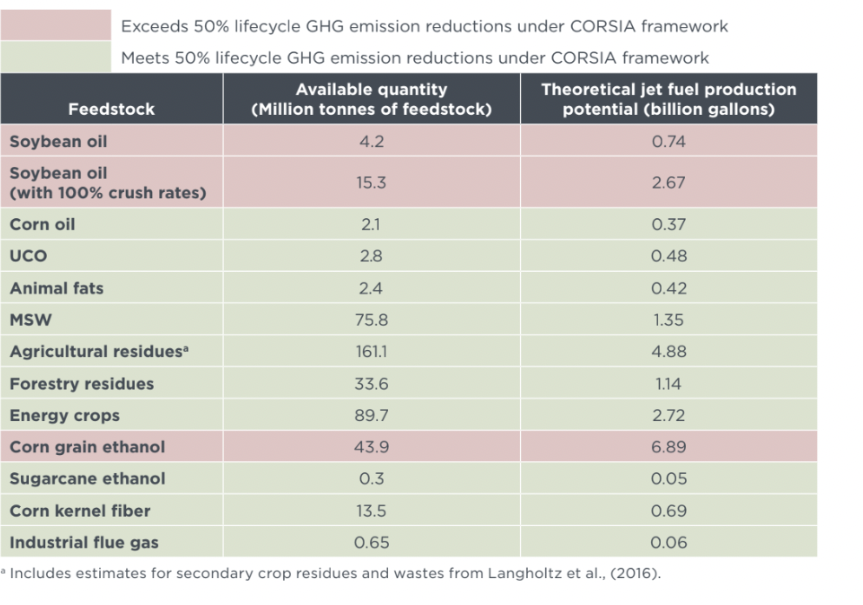
\includegraphics[width=0.8\textwidth]{Figure 10.png} % Replace 'fig10.png' with the path to your image file
\caption{Total theoretical U.S. SAF production potential by 2050 reproduced from O’Malley et al. 2023}
\label{fig:figure10}
\end{figure}

\section{Modeling Approach and Data}

\subsection{Approach}

This LCA study uses a cradle-to-grave assessment model, encompassing feedstock cultivation, production processes, transportation, and fuel combustion. The data for SAF pathways were sourced from the latest version of the greenhouse gasses, regulated emissions, and energy use in transportation (GREET) model using inputs and assumptions from peer-reviewed sources.  A comparative life-cycle assessment will be conducted between conventional Jet A1 kerosene, ATJ SAF from corn feedstock, HEFA SAF from used cooking oil feedstock, and FT SAF from municipal waste feedstock using the updated (2024) version of the GREET model. The study assumes a 50\% SAF blend with conventional jet fuel, reflecting the industry’s current blend percentage. The functional unit for the project is gCO2e/MJ for GHG emissions and MJ/MJ for energy consumption.

\subsection{Model}

Domestic and international organizations have developed models to quantify SAF's life-cycle greenhouse gas emissions. These models have been employed to inform government policies, business investment, and tax incentives. The greenhouse gasses, regulated emissions, and energy use in transportation (GREET) model is widely used in the United States. The California GREET model has been adopted by the California Air Resources Board to model California-specific emission considerations. Internationally, the International Civil Aviation Organization has developed the Carbon Offsetting and Reduction Scheme for International Aviation (CORSIA) model to similarly model the life-cycle emissions of aviation. 

\subsubsection{Argonne National Laboratory’s GREET Model}

Argonne National Laboratory has developed the greenhouse gasses, regulated emissions, and energy use in transportation (GREET) model to calculate the life-cycle of greenhouse gas emissions of various vehicle and fuel combinations. The model’s system boundary was expanded to include the well-to-wake analysis of aviation fuels and aircraft emissions for each unit of energy consumed by the aircraft or each unit of distance traveled (Elgowainy et al. 2012). The model includes the FT jet fuel from natural gas, coal, and biomass, bio-jet fuel from fast pyrolysis of cellulosic biomass, and HEFA from vegetable and algal oils (Elgowainy et al. 2012). Some of the latest updates to the GREET v1.3.0.14168 applicable to this project are a new pathway for FT SAF, life-cycle inventory of fertilizer and herbicide production, well-to-wheel life-cycle assessment of large agricultural tractor, and light-, medium-, and heavy-duty vehicles’ mass and characteristics (Wang et al. 2023).

\subsubsection{Argonne National Laboratory’s 40BSAF-GREET 2024 Model
}
Recently, the 40BSAF-GREET 2024 was released in April 2024 and last updated in October 2024 to examine SAF production pathways to calculate reductions in GHG emissions for eligibility for the 40B tax credit (U.S. Department of Energy 2024). The Inflation Reduction Act of 2022 established the Sustainable Aviation Fuel Credit. This tax credit applies to SAF sold or used during the calendar year 2024 that meets a minimum reduction of 50\% in life-cycle GHG emissions with higher credit rates available for further reductions (U.S. Department of Energy 2024). The system boundary of the 40BSAF-GREET 2024 model includes all greenhouse emissions related to SAF production, from feedstock growth, feedstock processing, SAF production, fuel blending, and final use. The boundary also includes indirect emissions from production and transportation, as detailed below. 

\begin{figure}[H]
\centering
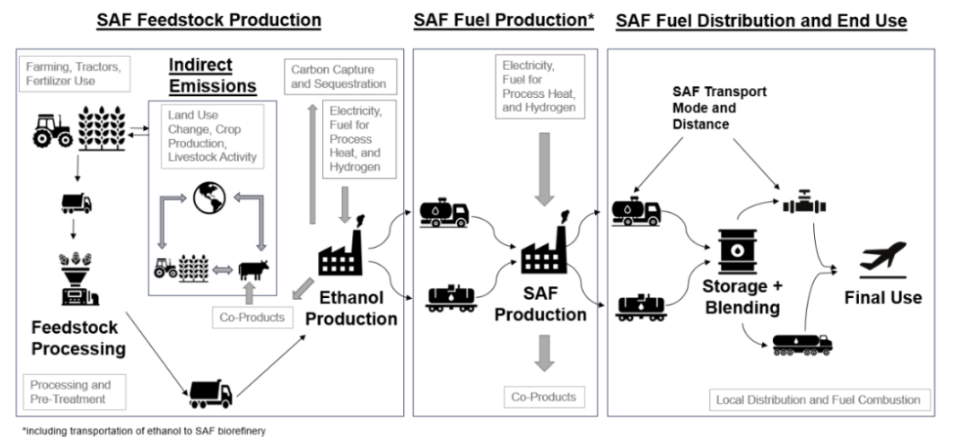
\includegraphics[width=0.8\textwidth]{Figure 11.png} % Replace 'fig10.png' with the path to your image file
\caption{SAF production GREET system boundary reproduced from U.S. Department of Energy 2024}
\label{fig:figure11}
\end{figure}

The functional unit of the model is 1 mega Joule (MJ) of fuel on the lower heating value. The calculated GHG emissions for the SAF are compared to a baseline of 89 gCO2e/MJ of conventional aviation fuel. The model assumes that one gallon of SAF equals the lower heating value of 126.37 MJ. Once the GHG emissions reduction is found, the model enables the user to claim the tax credit based on the gallons of SAF produced (U.S. Department of Energy 2024). The model uses the Intergovernmental Panel on Climate Change’s (IPCC) 100-year global warming potential of carbon dioxide (CO2), methane (CH4), and nitrous oxides (N2O) to determine the grams of CO2e produced per MJ of SAF produced (U.S. Department of Energy 2024). The model only calculates GHG emissions from the HEFA and ATJ, from ethanol feedstock, and production methods from seven distinct pathways produced in the United States but exempts Canadian canola and rapeseed and Brazilian sugarcane from the domestic production requirement (U.S. Department of Energy 2024). 
Additionally, there is no origin restriction on the tallow and used cooking oil feedstocks. However, the entire life-cycle of the feedstocks is still required, which may dissuade feedstocks with a high transportation impact (U.S. Department of Energy 2024). 


An important assumption of the GREET model is that CO2 emissions from biogenic fuels are assumed to be offset entirely during the growth of biomass feedstock (U.S. Department of Energy 2024). Thus, the calculated value for the combustion stage only includes the non-CO2 emissions from an aircraft, which is typically insignificant in magnitude relative to emissions in other stages. This assumption is similar to ICAO’s CORSIA model and is consistent with the IPCC Fifth Assessment Report (ICAO 2022). 

\subsection{Data}

Life-cycle assessments of sustainable aviation fuels often rely on data from the GREET model developed by the Argonne National Laboratory. One key feature of GREET is that it allows users to adjust various assumptions and parameters, such as land-use changes, feedstock types, energy inputs, and conversion efficiencies, which can significantly affect the final emission estimates. While this flexibility helps assess a wide range of biofuels and scenarios, it results in varying emissions data. On the other hand, the GREET model is a powerful tool for sensitivity analysis. For this study, the GREET model will test different combinations of SAF feedstocks and production locations within the United States.

\subsubsection{HEFA}

Parameters for producing HEFA SAF from the used cooking oil (UCO) feedstock are sourced from Mannion et al.’s (2024) methodology for modeling the life-cycle emissions from chemical mass and energy balance included Table 2. Their study imposed the following constraints on the yield of SAF: the chemical composition of the UCO, the required ASTM chemical properties of HEFA SAF, and an elemental mass and energy-conserved reaction (Mannion et. al 2024).  The study’s results agreed with the GREET model when the same assumptions were entered into the model  (Mannion et. al 2024). This LCA was selected to model the realistic yield of SAF from UCO at a generic production facility in the 40BSAF-GREET model. The value for SAF produced consists of the HEFA SAF produced and associated coproducts (naphtha, propane, and diesel). The mass breakdown of these individual products is included in Figure 10.

The following are specific assumptions for the HEFA pathway in this study. The energy is assumed to be sourced solely from the electricity grid with no onsite burning of natural gas. Hydrogen is produced offsite and transported to the SAF production facility for this scenario. Lastly, the GREET model uses estimated national averages for the transport distances and modes for soybean oil, canola/rapeseed oil, and waste oils and fats used in HEFA production facilities (U.S. Department of Energy 2024).

\begin{table}[H]
\centering
\begin{tabular}{|l|r|l|}
\hline
\multicolumn{3}{|c|}{\textbf{SAF Production}} \\
\hline
\textbf{Parameter} & \textbf{Value} & \textbf{Unit} \\
\hline
SAF Produced & 48.83 & kg \\
Feedstock: UCO Consumption & 100 & kg \\
Grid Electricity & 492.3 & MJ \\
Offsite, fossil NG-derived H$_2$ Consumption & 2.44 & kg \\
\hline
\end{tabular}
\caption{HEFA SAF production parameters adapted from Mannion et al. 2024.}
\label{tab:saf_production}
\end{table}
\begin{table}[H]
\centering
\begin{tabular}{|l|r|}
\hline
\multicolumn{2}{|c|}{\textbf{Inputs}} \\
\hline
\textbf{Parameter} & \textbf{Mass (kg)} \\
\hline
Raw Used Cooking Oil & 100.00 \\
Hydrogen & 4.00 \\
\hline
\textbf{Total} & \textbf{104.00} \\
\hline
\end{tabular}

\begin{tabular}{|l|r|}
\hline
\multicolumn{2}{|c|}{\textbf{Outputs}} \\
\hline
\textbf{Parameter} & \textbf{Mass (kg)} \\
\hline
Residue & 0.50 \\
Water & 6.16 \\
Excess Hydrogen & 1.56 \\
Carbon Monoxide & 0.28 \\
Carbon Dioxide & 10.00 \\
C$_3$ (Propane) & 4.05 \\
C$_4$--C$_8$ (Naphtha Range) & 21.02 \\
C$_9$--C$_{15}$ (Jet Range) & 48.83 \\
C$_{16}$--C$_{18}$ (Diesel Range) & 11.61 \\
\hline
\textbf{Total} & \textbf{104.00} \\
\hline
\end{tabular}

\begin{tabular}{|l|r|}
\hline
\textbf{HEFA-SPK Yield} & \textbf{48.83\%} \\
\hline
\end{tabular}

\caption{Mass balance inputs to convert UCO to HEFA SAF reproduced from Mannion et al. 2024.}
\label{tab:saf_production}
\end{table}


\subsubsection{ATJ}

The emission values associated with ATJ are calculated via the GREET model in the Staples et al. (2014) study. The assumptions associated with ATJ are summarized below:

\begin{table}[h!]
\centering
\begin{tabular}{|p{4cm}|p{8cm}|}
\hline
\textbf{Parameter} & \textbf{Value / Description} \\
\hline
Fermentation & 90\% Saccharification Efficiency \\
\hline
Grid & Grid average carbon intensity of transported U.S. electricity from GREET, 670.0 gCO2e/kWh \\
\hline
\end{tabular}
\caption{Corn ATJ Assumptions adapted from Staples et al. 2014}
\label{tab:fermentation_grid}
\end{table}

\begin{table}[H]
\centering
\resizebox{\textwidth}{!}{ % Resize to fit the text width
\begin{tabular}{|l|c|c|c|c|c|c|c|c|c|}
\hline
\textbf{Study/year} & \textbf{Corn yield} & \textbf{Nitrogen} & \textbf{Nitrogen} & \textbf{Corn ethanol} & \textbf{Ethanol} & \textbf{Total\footnotemark[1]} & \textbf{Coproduc-} & \textbf{Net\footnotemark[1]} \\
                    & \textbf{(Bu/acre)} & \textbf{fertilizer} & \textbf{fertilizer} & \textbf{conversion} & \textbf{conversion} & \textbf{energy} & \textbf{products\footnotemark[1]} & \textbf{energy} \\
                    &                    & \textbf{application} & \textbf{production} & \textbf{rate}       & \textbf{process}   & \textbf{use}   & \textbf{energy} & \textbf{value} \\
                    &                    & \textbf{rate (lb/acre)} & \textbf{(Btu/lb)} & \textbf{(gal/bu)} & \textbf{(Btu/gal)} & \textbf{(Btu/gal)} & \textbf{credits (Btu/gal)} & \textbf{(Btu/gal)} \\
\hline
Pimentel (1991) & 110 & 136 & 37,551 & 2.50 & 73,687 & 131,017 (LHV) & 21,500 & -33,517 \\
Pimentel (2001) & 127 & 129 & 33,547 & 2.50 & 75,118 & 131,062 (LHV) & 21,500 & -33,562 \\
Keeney and DeLuca (1992) & 119 & 135 & 37,958 & 2.56 & 48,470 & 91,196 (LHV) & 8,078 & -8,438 \\
Marland and Turhollow (1990) & 119 & 127 & 31,135 & 2.50 & 50,105 & 73,934 (HHV) & 8,127 & 18,154 \\
Lorenz and Morris (1995) & 120 & 123 & 27,605 & 2.55 & 53,956 & 81,090 (HHV) & 27,579 & 30,589 \\
Ho (1989) & 90 & NR & NR & NR & 57,000 & 90,000 (LHV) & 10,500 & -4,000 \\
Wang et al. (1999) & 125 & 131 & 21,092 & 2.55 & 40,850 & 68,450 (LHV) & 14,950 & 22,500 \\
Agri. and Agri-Food Canada (1999) & 116 & 125 & NR & 2.69 & 50,415 & 68,450 (LHV) & 14,055 & 29,826 \\
Shapouri et al. (1995) & 122 & 125 & 22,159 & 2.53 & 53,277 & 82,824 (HHV) & 15,056 & 16,193 \\
This study (2002) & 125 & 129 & 18,392 & 2.66 & 51,779 & 77,228 (HHV) & 14,372 & 21,105 \\
\hline
\end{tabular}
}
\caption{Energy Input Assumptions of Corn Ethanol Studies Reproduced from Shapouri et al. 2002}
\footnotetext[1]{The midpoint or average is used when studies report a range of values.}

\footnotetext{NR: Not reported.}

\footnotetext{LHV: Low heat value = 76,000 Btu per gallon of ethanol. Keeney and DeLuca used 74,680 Btu per gallon of ethanol. HHV: High heat value = 83,961 Btu per gallon of ethanol. Lorenz and Morris used 84,100 Btu per gallon of ethanol.}
\end{table}

\subsubsection{FT}

For FT, model inputs were obtained from Suresh et al. (2018). The study used Monte Carlo analysis, and below is a chart of parameters distribution. 

\begin{figure}[H]
    \centering
    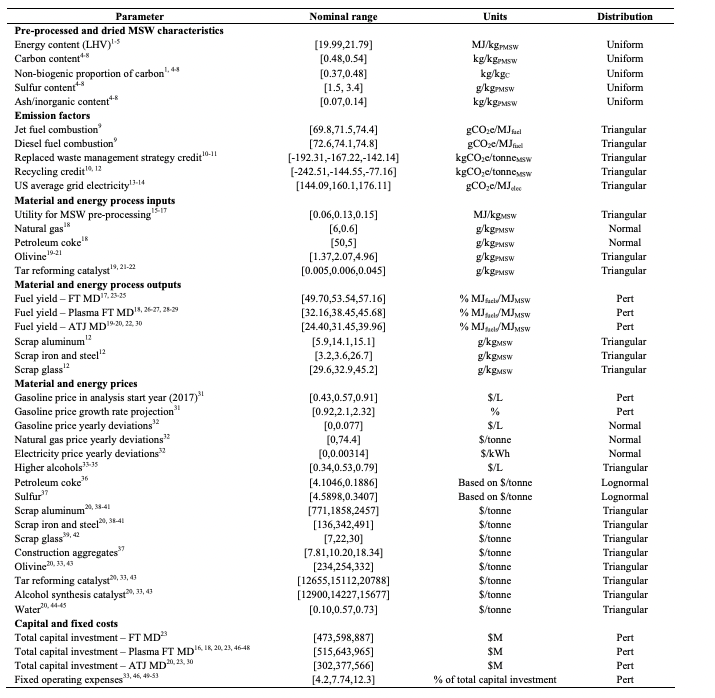
\includegraphics[width=0.8\textwidth]{FT Data.png} % Replace 'filename.png' with the name of your image file
    \caption{Model Inputs for FT adapted from Suresh et al. 2018}
    \label{fig:Fisher} % Replace 'yourlabel' with a unique identifier for referencing the figure
\end{figure}




\section{Results and Findings}

\section{Sensitivity Analysis}

\section{Uncertainty Assessment and Management}

\section{Interpretation and Discussion of Results}

\section{Conclusions and Recommendations}

\section{References}

\begin{description}
    \setlength{\itemsep}{0pt} % Reduces space between items
    \small % Optional: Reduces font size for better fit

    \item Aui, A., Wang, Y., and Mba-Wright, M. (2024). “Evaluating the economic feasibility of cellulosic ethanol: A meta-analysis of techno-economic analysis studies.” \textit{Renewable and Sustainability Energy Reviews}, 145, 1–15. \url{https://doi.org/10.1016/j.rser.2021.111098}
    
    \item Bergero, C., Gosnell, G., Gielen, D., Kang, S., Bazilian, M., and Davis, S. J. (2023). "Pathways to net-zero emissions from aviation." \textit{Nature Sustainability}, 6, 404–414. \url{https://doi.org/10.1038/s41893-022-01046-9}
    
    \item Calderon, O. R., Tao, L., Abdullah, Z., Talmadge, M., Milbrandt, A., Smolinski, S., Moriarty, K., Bhatt, A., Zhang, Y., Ravi, V., Skangos, C., Davis, R., and Payne C. (2024). “Sustainable Aviation Fuel State-of-Industry Report: Hydroprocessed Esters and Fatty Acids Pathway.” \textit{National Renewable Energy Laboratory}. \url{https://www.nrel.gov/docs/fy24osti/87803.pdf}, Accessed 10/14/2024 at 12:16 PM
    
    \item Cui, Q. and Lei, Y. (2023). "Pathways analysis to reducing aircraft emissions for China-Foreign routes." \textit{npj Climate Action}, 2, 1–9. \url{https://doi.org/10.1038/s44168-023-00047-4}
    
    \item de Jong, S., Antonissen, K., Hoefnagels, R., Lonza, L., Wang, M., Faaij, A., and Junginger, M. (2017). “Life-cycle analysis of greenhouse gas emissions from renewable jet fuel production.” \textit{Biotechnology for Biofuels}, 10(64), 1–18. \url{https://doi.org/10.1186/s13068-017-0739-7}
    
    \item Dray, L., Schäfer, A. W., Grobler, C., Falter, C., Allroggen, F., Stettler, M. E. J., & Barrett, S. R. H. (2022). “Cost and emissions pathways towards net-zero climate impacts in aviation.” \textit{Nature Climate Change}, 12(10), 956–962. \url{https://doi.org/10.1038/s41558-022-01485-4}
    
    \item Elgowainy, A., Han, J., Wang, M., Carter, N., Stratton, R., Hilemann, J., Malwitx, A., Balasubramanian, S. (2012). “Life-Cycle Analysis of Alternative Aviation Fuels in GREET.” \textit{Argonne National Laboratory}. \url{https://publications.anl.gov/anlpubs/2016/05/127787.pdf}, Accessed 10/2/2024 at 3:43 PM
    \item
    EXP (2023). “Municipal Solid Waste to Fuel Study: Municpal Port of Seattle + King Country Solid Waste Division.” \url{https://your.kingcounty.gov/dnrp/library/solid-waste/Solid-waste-planning-monitoring/Solid-waste-monitoring/MSW-fuels-study.pdf}, Accessed 10/20/2024 at 11:01 AM.
    \item Han, J., Tao, L., and Wang, M. (2017). “Well-to-wake analysis of ethanol-to-jet and sugar-to-jet pathways.” \textit{Biotechnology for Biofuels}, 10, 1–15. \url{https://doi.org/10.1186/s13068-017-0698-z}
    
    \item International Civil Air Organization (2022). “CORSIA Eligible Fuels – Life Cycle Assessment Methodology.” \url{https://www.icao.int/environmental-protection/CORSIA/Documents/CORSIA_Eligible_Fuels/CORSIA_Supporting_Document_CORSIA%20Eligible%20Fuels_LCA_Methodology_V5.pdf}, Accessed 10/24/2024 at 10:53 AM
    
    \item International Energy Agency (2019). “The Future of Hydrogen.” \url{https://www.iea.org/reports/the-future-of-hydrogen}, Accessed 10/23/2024 at 4:10 PM.
\end{description}
\begin{description}
    \setlength{\itemsep}{0pt} % Reduces space between items
    \small % Optional: Reduces font size for better fit

    \item International Aviation Trade Association (2024). “Energy and New Fuels Infrastructure: Net Zero Roadmap.” \url{https://www.iata.org/contentassets/8d19e716636a47c184e7221c77563903/energy-and-new-fuels-infrastructure-net-zero-roadmap.pdf}, Accessed 10/25/2024 at 11:53 AM

\item[] Jing, L., El-Houjeiri, H.M., Monfort, J.C., Littlefield, J., Al-Qahtani, A., Dixit, Y., Speth, R. L., Brandt, A. R., Masnadi, M. S., MacLean, K. L., Peltier, W., Gordon, D., and Bergerson, J. A. (2022). "Understanding variability in petroleum jet fuel life cycle greenhouse gas emissions to inform aviation decarbonization." \textit{Nature Communications}, 13, 1–10. \url{https://doi.org/10.1038/s41467-022-35392-1}, Accessed 10/10/2024 at 3:00 PM]
    
    \item Lau, J. I. C., Wang, Y. S., Ang, T., Seo, J. C. F., Khadaroo, S. N. B. A., Chew, J. J., Lup A. N. K., and Sunarso J. (2024). “Emerging technologies, policies and challenges toward implementing sustainable aviation fuel (SAF).” \textit{Biomass and Bioenergy}, 186, 1–29. \url{https://doi.org/10.1016/j.biombioe.2024.107277}
    
    \item Mannion, L. A., Redington, C., Kelly, M., Bell, A., and Dooley, S. (2024). “The effect of used cooking oil composition on the specific CO2e emissions embodied in HEFA-SPK production.” \textit{Biofuels, Bioproducts and Biorefining}, 18(4), 837–854. \url{https://doi.org/10.1002/bbb.2653}
    
    \item Mannion, L. A., Bell, A., Watson-Murphy, T., Kelly, M., Ghaani, M. R., and Dooley, S. (2024). “A physics constrained methodology for the life cycle assessment of sustainable aviation fuel production.” \textit{Biomass and Bioenergy}, 185, 1–18. \url{https://doi.org/10.1016/j.biombioe.2024.107169}
    
    \item Merchant, N., Kent, E., and Lewis, J. (2022). “Decarbonizing aviation: Challenges and opportunities for emerging fuels.” \textit{Clean Air Task Force}. \url{https://www.catf.us/resource/decarbonizing-aviation-challenges-and-opportunities-for-emerging-fuels/}, Accessed 10/10/2024 at 8:26 AM
    
    \item Office of Energy Efficiency & Renewable Energy (2024). “Sustainable Aviation Fuel Grand Challenge: Tracking Metrics and Mid-2024 Dashboard.” \url{https://biomassboard.gov/sustainable-aviation-fuel-grand-challenge-progress}, Accessed 10/6/2024 at 5:10 PM
    
    \item O’Malley, J., Pavlenko, N., and Kim, Y. H. (2023). “Meeting the SAF Grand Challenge: Current and Future Measures to Increase U.S. Sustainable Aviation Fuel Production Capacity.” \textit{The International Council on Clean Transportation}. \url{https://theicct.org/publication/us-saf-production-capacity-nov23/}, Accessed 10/23/2024 at 5:40 PM

    \item Pressley, P. N., Aziz, T. N., DeCarolis, J. F., Barlaz, M. A., He, F., Li, F., and Damgaard, A. (2014), “Municipal solid waste conversion to transportation fuels: a life-cycle estimation of global warming potential and energy consumption.” \textit{Journal of Cleaner Production}, 70, 145–153. \url{https://doi.org/10.1016/j.jclepro.2014.02.041}
    
    \item Sacchi, R., Becattini, V., Gabrielli, P., Cox, B., Dirnaichner, A., Bauer, C., and Mazzotti, M. (2023), “How to make climate-neutral aviation fly.” \textit{Nature Communications}, 14, 1–17. \url{https://doi.org/10.1038/s41467-023-39749-y}
    
    \item Shapouri, H., Duffield, J. A., and Wang, M. (2002), “The Energy Balance of Corn Ethanol: An Update.” \textit{United States Department of Agriculture, Agricultural Economic Report No. 813}. \url{https://www1.eere.energy.gov/bioenergy/pdfs/energy_balance_of_corn_ethanol.pdf}, Accessed 10/24/2024 at 4:00 PM
    
    \item Staples, M. D., Malina, R., Olcay, H., Pearlson, M. N., Hileman, J. I., Boies, A., and Barrett, S. R. (2014). “Life-cycle greenhouse gas footprint and minimum selling price of renewable diesel and jet fuel from fermentation and advanced fermentation production technologies.” \textit{Energy & Environmental Science}, 7, 1545–1554. \url{https://doi.org/10.1039/C3EE43655A}

    \item Suresh, P., Malina, R., Staples, M. D., Lizin, S., Olcay, H., Blazy, D., Pearlson, M. N., and Barrett, S. R. H. (2018). “Environmental Science & Technology.” \textit{Environmental Science & Technology}, 52(21), 12055–12065. \url{https://doi.org/10.1021/acs.est.7b04277}
    
    \item U.S. Department of Energy (2024). “Guidelines to Determine Life Cycle Greenhouse Gas Emissions of Sustainable Aviation Fuel Production Pathways using 40BSAF-GREET 2024.” \url{https://www.energy.gov/sites/default/files/2024-04/40bsaf-greet_user-manual.pdf}, Accessed 9/13/2024 at 12:14 PM
    \item[]  
    U.S. Environmental Protection Agency (n.d.), “Basic Information about Landfill Gas.” \href{https://www.epa.gov/lmop/basic-information-about-landfill-gas}{https://www.epa.gov/lmop/basic-information-about-landfill-gas}, Accessed 10/15/2024 at 11:30 AM
\item[]  
   U.S. Environmental Protection Agency (n.d.), “National Overview: Facts and Figures on Materials, Wastes and Recycling.” \href{https://www.epa.gov/facts-and-figures-about-materials-waste-and-recycling/national-overview-facts-and-figures-materials}{https://www.epa.gov/facts-and-figures-about-materials-waste-and-recycling/national-overview-facts-and-figures-materials}, Accessed 10/15/2024 at 11:36 AM 
    \item U.S. Government Accountability Office (2023). “Sustainable Aviation Fuel: Agencies Should Track Progress towards Ambitious Federal Goals.” Report to Congressional Committees, GAO-23-105300. \url{https://www.gao.gov/assets/d23105300.pdf}, Accessed 10/25/2024 at 10:59 AM
    \item Wang, M., Cai, H., Lee, U., Kar, S., Sykora, T., and Liu, X. (2024). “Development of R&D GREET 2023 Rev1 to Estimate Greenhouse Gas Emissions of Sustainable Aviation Fuels for 40B Provision of the Inflation Reduction Act.” \textit{Argonne National Laboratory}. \url{https://doi.org/10.2172/2348933}, Accessed 10/4/2024 at 12:20 PM
    
    \item Wang, F., & Rijal, D. (2024). “Sustainable Aviation Fuels for Clean Skies: Exploring the Potential and Perspectives of Strained Hydrocarbons.” \textit{Energy & Fuels}, 38(6), 4904–4920. \url{https://doi.org/10.1021/acs.energyfuels.3c04935}
    
\end{description}


\end{document}
